\begin{frame}
\frametitle{Contd.}

\setlength{\columnsep}{10pt}
\begin{multicols}{2}
\setlength{\leftmargin}{1pt}
\setlength{\rightmargin}{0pt}
\begin{figure}
    \centering
    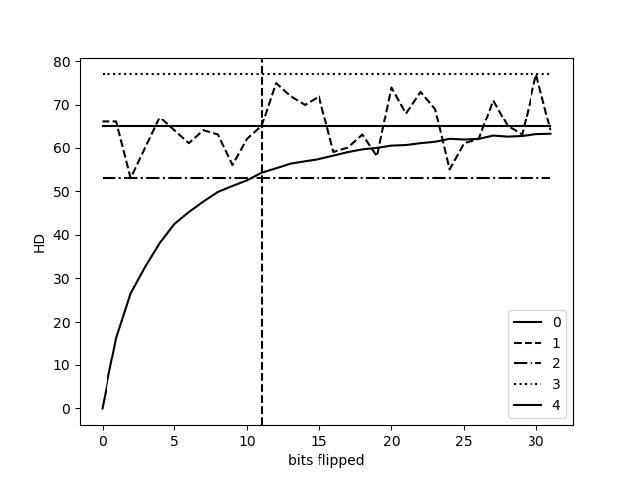
\includegraphics[scale=0.55]{fig2.jpg}
    \caption{Averaging of effects on $Y$ when bits are 
flipped in $X$.}
\end{figure}

\columnbreak
Legend of the Plot : 
\begin{enumerate}
    \setcounter{enumi}{-1} % Set the counter to start from 0
    \item \footnotesize{$HD(X^\prime, Y^\prime)$ as $n$ bits in $X^\prime$ are flipped.}
    \item \footnotesize{$HD(X,Y)$ of random $X$s}
    \item \footnotesize{\textit{Minimum expected difference} between two random $X$s}
    \item \footnotesize{\textit{Maximum expected difference} between two random $X$s}
    \item \footnotesize{\textit{Expected average difference} between two random $X$s}
    \item[] \footnotesize{The vertical line is where the bits flipped needed for the Hamming distance to be within the range of expected random distances}
\end{enumerate}
\end{multicols}
\end{frame}